\section{Background}
% From the Project Proposal marking sheet:
%   - Demonstrate a masterful understanding of the material in the topic area. 
%   - Your selection of source material should be very descriminating. 
%   - Your background should be most helpful in understanding 
%   the rest of the document.
%
% Your background should introduce all relevant technical details such that
% a lay-person will understand the problem space and how your proposed solution
% will contribute.

\subsection{Software Testing}

\subsubsection{Regression Testing}

In software engineering, the most commonly used method of software testing would be regression testing. Regression testing revoles around 
identifying parts of the program that is changed and verifying their behavior through a test suite; e.g. Unit, System, and Integration-level tests
\cite{testing}. Thus, that would verify whether the program behaves as intended or not.

In practice, regression testing would be limited to the capabilities of humans to define the behavior of the program. As such, there is an inherent 
risk of errors happening due to human mistakes; as it's possible that the defined behavior is not correct. Defining the complete set of behavior 
of the intended program through testing requires developers to spend a considerable amount of time to write tests manually \cite{differentialTesting}. 

As such, \textbf{random testing} is introduced to substitute humans with deterministic computer behaviors.

\subsubsection{Random Testing}

Random testing is a suite of random tests generated by the computer to determine the correctness of the program based on a predetermined 
set of rules \cite{differentialTesting}. For example, \cite[Sec. 2]{randomTesting} would generate test cases and 
execute them on programs which have a predictable result. For instance, if a program would deviate from the expected results, then the 
program would have undefined behaviors in them.

The difficulty of random testing lies in determining the set of rules to generate test cases. In \cite{differentialTesting}, the test cases 
are generated by substituting the subset of the input to a random input. While this allows test cases to be generated quickly, programs would only 
need several \emph{"interesting values"} or edge cases to consider in their behavior. As such, a stronger test suite such as an 
\textbf{inference-based test generation} would be preferrable in this project.

\subsubsection{Inference-based Exhaustive Testing}
\label{sec:inferenceTesting}

Exhaustive tests such as \cite{isabelleQuickcheck} takes into account the possible variable bounds of a program and converts it to a set of 
inference rules. For a program to be correct, all of the premises \emph{(P, Q)} in the inference rules \emph{(P \rightarrow Q)} must be correct. As 
such, finding a counterexample would be as simple as determining if the bounds of a variable would result in a satisfiable \emph{\lnot(P \rightarrow Q)}. 
This could be extended even further by checking the inference rules on a SAT solver to find premises where the inference rules would be incorrect 
\cite[Ch. 5]{isabelleProof}. Exhaustive searching allows developers to only focus on defining the behavior of the program, rather than defining 
tests to define the behavior.

\subsection{Isabelle}
\label{sec:Isabelle}

Isabelle is an interactive theorem prover that utilizes multitude of tools towards automatic proving. It emphasizes breaking down a proof 
for a theorem towards multiple smaller goals that are achievable called tactics. Tactics are functions written in the implementation of Isabelle 
that works on a proof state \cite{isabelleProof}. It either outputs a direct proof towards the goal, or breaks it down into more smaller sub-goals 
in a divide-and-conquer manner. These tactics work on the foundation that theory definitions can be modified into a set of inference rules that 
could be automatically reasoned with by the system.

Finding the right proving methods and arguments to utilise is one of the biggest issues for proving a theorem \cite{isabelleProof}. There are 
many tools in Isabelle's arsenal that can help the user progress towards their proof \cite{IsabelleHOL}. However, the most notable ones are 
Sledgehammer, Quickcheck, and Nitpick.

\subsubsection{Sledgehammer}
\label{sec:Sledgehammer}

Sledgehammer is one of the tools in Isabelle that \emph{could} automatically prove a theorem. It utilizes the set of inference rules as 
conjectures which can be cross-referenced with relevant facts (lemmas, definitions, or axioms) from Isabelle \cite[Sec. 3]{isabelleProof}. 
Afterwards, Sledgehammer passes them into resolution provers and SMT solvers which tries to solve it \cite[Sec. 3.3]{isabelleProof}. If a reasonable 
proof is found, Sledgehammer would then reconstruct the inference rules back into a \emph{relatively} human-readable proof definition in the style of 
Isabelle/Isar \cite[Sec. 3.4]{isabelleProof}.

Utilizing Sledgehammer has been proven to be an effective method of theorem proving. Sledgehammer, combined with external SMT solvers, could 
solve 60.1\% of proof goals, with a 44.7\% success rate for non-trivial goals \cite[Sec. 6]{isabelleSledgehammerSMT}. Despite their 
potential, as Blanchette et al. notes \cite[pp. 2]{isabelleProof}:

\begin{quote}
    "\dots most automatic proof tools are helpless in the face of an invalid conjecture. Novices and experts alike can enter invalid formulas and 
    find themselves wasting hours (or days) on an impossible proof; once they identify and correct the error, the proof is often easy."
\end{quote}

To make it easier for users to avoid this trap, Isabelle complements automatic theory proving with counterexample generators such as Quickcheck 
and Nitpick.

\subsubsection{Quickcheck}
\label{sec:Quickcheck}

Quickcheck is one of the counterexample generators in Isabelle. It works by utilizing code generation features of Isabelle by translating 
conjectures into ML (or Haskell) code \cite{isabelleQuickcheck}. This allows Quickcheck to discover counterexamples quickly by assiging 
free variables on the code via random, exhaustive, or narrowing test data generators. However, this would also mean that Quickcheck is limited 
to \emph{executable} and \emph{some} well defined unbounded proof definitions \cite{isabelleQuickcheck}.

Random testing a conjecture assigns free variables with a pseudo-random values \cite[Sec. 3.1]{isabelleQuickcheck}. This strategy tends to be fast, 
with the ability to generate millions of test cases within seconds. However, random testing could easily overlook obvious counterexamples. 
Furthermore, random testing is also limited into proof definitions that are well defined \cite{isabelleQuickcheck}. As such, exhaustive and narrowing 
test data generators are more suitable for proof definitions that are non-trivial or have unbounded variables.

Exhaustive and narrowing test data generators systematically generates values up to their bounds \cite{isabelleQuickcheck}. 
However, exhaustive test data generators would fail to find counterexamples of proofs that have unbounded variables. Narrowing test data generators 
would improve on that by evaluating proof definitions symbolically rather than taking variables at face value. This is possible due to 
term rewriting static analysis done on the proof definitions \cite[Sec. 5]{isabelleQuickcheck}.

Based on observed results, Bulwahn notes that random, exhaustive, and narrowing testing are comparable in terms of performance; with 
exhaustive testing finding non-trivial counterexamples easily compared to random testing \cite[Sec. 7]{isabelleQuickcheck}. As much of the 
proof definitions are defined over unbounded variables, exhaustive testing are the default option for Quickcheck.

\subsubsection{Nitpick}
\label{sec:Nitpick}

An alternative to find counterexamples for proof definitions would be Nitpick. Instead of enumerating the bounds of free variables inside the 
system of Isabelle, Nitpick passes conjectures -- translation of proof definitions into inference rules -- into SAT solvers 
\cite[Sec. 5]{isabelleProof}. SAT solvers would then search for premises that would falsify the given conjecture. If a conjecture 
has bounds over finite domains, Nitpick would \emph{eventually} find the counterexample. Conjectures with unbounded variables would be partially 
evaluated \cite[Sec. 5.2]{isabelleProof}. However, it could not determine whether infinite bounds would result to a satisfiable conjecture.

Nitpick and Quickcheck shouldn't be compared to one another. Instead, they are are tools that should be used interchangeably to determine 
whether a conjecture would be possible to proof \cite{isabelleQuickcheck}. The performance of Nitpick are comparable to Quickcheck, with 
Nitpick being able to find counterexamples to proof definitions that are not executable within Isabelle's code generation 
\cite[Sec. 7]{isabelleQuickcheck}.

\subsection{Formal Verification of Compiler}

If software code is the recipe for system behaviors, then compilers would be the chef that puts it all together. Most people would assume that 
the behavior of compiled programs would match the input program exactly. However, this is usually not the case \cite{compcertVerification}. 
Chefs would have their own way of creating magical concoctions from a recipe, and so does a compiler. Not only does a compiler try to replicate 
system behaviors, it would try to make them faster in their own ways; i.e. adding optimizations or reducing unneeded behaviors. However, the 
original behavior of the program must be preserved in order to consider a compiler to be correct 
\cite{compcertVerification,AliveInLean,Alive2}, and \cite{Term_Graph_Optimizations}.

Validating compiler correctness is not easy. While the correctness of a compiler could be verified by defining behaviors through regression testing, 
it would be time consuming to do and not exactly productive \cite{randomTesting,compcertVerification}. There are multitude of ways that a 
compiler can go wrong \cite[Sec. 1.2]{CompilerOptimization}; all of which have their own specific way of verifying correctness. For example, 
CompCert \cite{compcertVerification} tries to tackle all of the implementation and semantics errors inside a compiler (See \ref{sec:CompCert}) -- 
creating a completely verified compiler for the C language platform. Formally verifying compilers in the scale of CompCert would require vast amounts 
of time and resources, which projects often don't have.

As such, there are smaller scale projects such as Alive \cite{AliveInLean} \& Alive2 \cite{Alive2} that focus on behavior translation errors 
in LLVM's peephole optimizer (See \ref{sec:Alive}). Veriopt tries to work on the same steps as CompCert -- by defining the IR of GraalVM and 
proving much of the side-effect-free data-flow behavior optimizations that occurs in GraalVM 
\cite{ATVA21_GraalVM_IR_Semantics,Term_Graph_Optimizations} (See \ref{sec:Veriopt}).

\subsubsection{CompCert}
\label{sec:CompCert}

CompCert verifies that Clight, a subset of C programming language \cite{compcertVerification}, is correct through several steps:
\begin{enumerate}
    \item 
    With deterministic programs, a compiler would compile a source program to the produced program -- in which both of the programs must have 
    the same behavior.
    
    This step is done by augmenting the compiler code with a \emph{certificate} -- code that carries proof that the behavior is exactly as intended 
    \cite[Sec. 2.2]{compcertVerification}.

    \item Compiler optimization phases must be accompanied by the formal definition of their Intermediate Representation (IR) semantics 
          \cite{compcertVerification,ATVA21_GraalVM_IR_Semantics}.
    
    \item Lastly, to formally verify each of the optimization phases, a compiler must either:
    \begin{enumerate}
        \item
        Prove that the code implementing the optimization is correct \cite[Sec. 2.4]{compcertVerification}.
        
        Veriopt uses this approach in verifying data-flow optimizations (See \ref{sec:Veriopt}).

        \item 
        Prove that the unverified code produce the correct behavior in their translation \cite[Sec. 2.4]{compcertVerification}.

        Alive uses this approach in verifying LLVM (See \ref{sec:Alive}).
    \end{enumerate}
\end{enumerate}

CompCert formally verifies each step in the source, intermediate, and target languages that goes through the compiler 
\cite[Sec. 3.3]{compcertVerification}. Furthermore, each code translation and optimization are accompanied by \emph{certificates} that prove 
the correctness of the semantics. This is done through Coq, a proof assistant similar to Isabelle. The workflow of Coq also remains closely related to 
Isabelle (See \ref{sec:Isabelle}) \cite[Sec. 3.3]{compcertVerification}. 

CompCert utilizes Coq not only to formally verify the semantics of Clight, but also to generate the verified parts of the compiler code 
\cite[Sec. 3.4]{compcertVerification}. The clever part of CompCert is that it utilizes the functional programming capabilities of Coq 
to automatically generate code. As such, it is able to write a compiler-compiler -- which is the 3rd step of compiler verification research 
\cite{CompilerOptimization}.

The formal verification of Clight results in 42000 lines of Coq -- approximately equivalent to 3 years of man-hours 
of work \cite[Sec. 3.3]{compcertVerification}. As you can see, replicating the results of CompCert would require an enormous amount of work.
Formal verifications such as Alive (See Sec. \ref{sec:Alive}) and Veriopt (See Sec. \ref{sec:Veriopt}) undertakes the smaller subset, 
namely 1st and 2nd step, of compiler verification research thread \cite{CompilerOptimization}.

\subsubsection{Alive}
\label{sec:Alive}

Alive tackles a subset of compiler verification by verifying that code optimizations inside LLVM are correct \cite{AliveInLean}. For example, 
a compiler would optimize \((LHS = x * 2) \sqsupseteq (RHS = x << 1)\) (\(RHS\) is a refinement of \(LHS\)). While this may seem trivial, there would 
be a lot of edge cases where the behavior translation might be incorrect; e.g. buffer overflows.

\begin{figure}[ht]
    \centering
    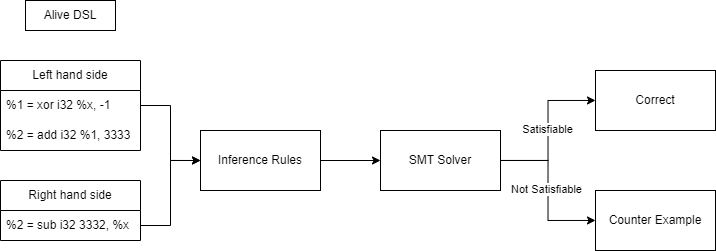
\includegraphics[width=0.8\textwidth]{Alive.png}
    \caption{How Alive verifies \((LHS = (X \oplus -1) + C) \sqsupseteq (RHS = (C-1) + X)\) \cite[pp. 1]{AliveInLean}}
    \label{fig:AliveSystem}
\end{figure}

To verify that code optimizations are correct, Alive utilizes inference-based exhaustive testing (See \ref{sec:inferenceTesting}) that allows 
the tool to encode machine code behaviors to inference rules. These inference rules are then passed to SMT solvers to check for their satisfiability 
(See Fig. \ref{fig:AliveSystem}). If the translation is proven to be correct, then it would mean that the underlying optimization code is correct.

Alive encodes LLVM's \cite{llvm} underlying IR semantics through their own DSL \cite[Fig. 1]{AliveInLean}. The DSL specification is made to be 
similar to LLVM's IR semantics to allow developers to easily integrate Alive with the development of DSL. This would represent the 
\emph{certificate} that the underlying optimization is formally verified to be correct.

Alive takes this further by creating Alive2: a system to translate LLVM IR into Alive's IR \cite{Alive2}. This allows the developers to entirely 
focus on developing LLVM, while completely ignoring the specifications of Alive. This has been found to be effective, as differential testing of 
LLVM's unit tests and Alive2 discovers multiple errors inside the unit test behaviors itself \cite[Sec. 8.2]{Alive2}. Alive \& Alive2 would cover 
the whole 1st and 2nd step of compiler optimizations research thread \cite[pp. 5]{CompilerOptimization}.

\subsubsection{Veriopt}
\label{sec:Veriopt}

In comparison to CompCert and Alive, the theoretical aspects of compiler verification are really similar. GraalVM's IR is made up of two components: 
control-flow nodes and data-flow nodes; which are combined as a sea-of-nodes data structure \cite{ATVA21_GraalVM_IR_Semantics}. However, 
Veriopt's DSL only concerns the subset of GraalVM's IR, which is the side-effect-free data-flow nodes \cite{Term_Graph_Optimizations}.
Side-effect-free data-flow nodes are comparatively easier to prove and optimize, as it would be considered defined -- as opposed to LLVM's undefined 
and poisoned variables \cite{Alive2}.

\begin{figure}[h]
    \emph{
        \textbf{optimization} InverseLeftSub: \((x - y) + y \longmapsto x\)
        \begin{description}[font=\small]
            \item[Termination Proof Obligation] \(trm(x) < trm(BinaryExpr BinAdd (BinaryExpr BinSub x y) y)\)
            \item[Refinement Proof Obligation] BinaryExpr BinAdd (BinaryExpr BinSub x y) y \sqsupseteq x
        \end{description}
    }

    \caption{Sample of Veriopt's DSL \cite[Fig. 3]{Term_Graph_Optimizations}}
    \todo[inline]{fix this formatting}
    \label{fig:VerioptDSLSample}
\end{figure}

Figure \ref{fig:VerioptDSLSample} defines the structure of DSL for an optimization phase. The \emph{\textbf{optimization}} keyword represent 
the proof definition that must be proven in Isabelle. Note that there are 2 proof obligations that must be met in order to consider that the 
side-effect-free optimization is correct: proof that the optimization phase would terminate; proof that each pass of the optimization phase would 
result in a refinement of the expression \cite{Term_Graph_Optimizations}. Note that these proofs would need to be provided by the users.

Currently, there's some tools that the developers of GraalVM could use to provide a \emph{certificate} towards the compiler code 
\cite[Sec. 7]{Term_Graph_Optimizations}. A semi-automated approach exists in a form of source code annotations \cite[Sec. 5.1]{Term_Graph_Optimizations}.
However, integrating new behaviors which would require new \emph{certificates} would be challenging, as the approach would only describe the behavior 
of the code -- instead of formally proving that the behavior is indeed correct.

Providing proof obligations for an optimization phase would be challenging for developers who are not \emph{experts in program verification}. Veriopt's 
DSL are implemented in Isabelle \cite{IsabelleHOL}, which comes with tools that assist in proving higher order logic (See \ref{sec:Isabelle}). 
However, using such tools would require the developers of GraalVM to be familiar with Isabelle -- something that ideally Veriopt would like to avoid. 
Similar tools such as Alive \cite{AliveInLean} would be preferrable. Hence, that's where this project would like to contribute.